\section{Performance}
\subsection{Improvements}

To establish the performance of the final code, we compare the results to a baseline code. This baseline code is our solution developed for the first assignment. Buses travel according to one fixed schedule, picking up and dropping off passengers. In the final code, we implemented all the improvements explained in Section \ref{sec:conceptual}. Table \ref{table:table1} shows the comparison between the baseline code and the final code.

\begin{table*}[htbp]
\centering
\begin{tabular}{ |c|c|c|  }
 \hline
  Measurement & Baseline & Final Code \\
 \hline
  Avg travel time & 150.01 & 72.53 \\
  Buses' expenses & 1039682 & 711251 \\
  Messages sent & 0 & 285  \\
  Final amount waiting & 232 & 25 \\
  Avg travel time remaining & 100.25 & 78.12 \\
  Final avg travel time & 156.34 & 75.48 \\
 \hline
\end{tabular}
\label{table:table1}
\caption{Performance results}
\end{table*}

Table \ref{table:table1} shows that there is a significant decrease of the costs. Not only does the travelling time and the amount of people waiting go down, the financial costs also lower. Solely the number of messages increase, because no communication system was implemented in the baseline version. 

These results highlights the advantages of an intelligent coordination and competition between buses. Because of transportation efficiency, travel time and passengers waiting are reduced, without increasing financial costs.

\subsection{Performance on test data}

Three data sets (\textit{day 1}, \textit{day 2} and \textit{day 4}) are available for testing our transportation system. Each data set contains data for a time span of 24 hours. Each 15 minutes, for each bus stop, the amount of travelers arriving and their destination is displayed. The day 1 data set is used to create our solution, whereas day 4 and day 5 are to test the proposal. In this section, we show the results of our solution for the three different data sets.

The final values of the different metrics for day 1, are shown in the right column of Table \ref{table:table1}. Figure \ref{fig:expense} shows the plot of the expenses, figure \ref{fig:messages} the messages send, figure \ref{fig:pass_waiting} the passengers waiting and figure \ref{fig:avg_tt} the travel time.

\begin{figure}[htbp]
\centering
\begin{minipage}{.48\textwidth}
  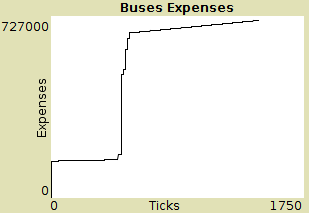
\includegraphics[width=\textwidth]{src/expenses.png}
  \caption{Expenses of the buses in Day 1.}
  \label{fig:expense}
\end{minipage}
\begin{minipage}{.48\textwidth}
  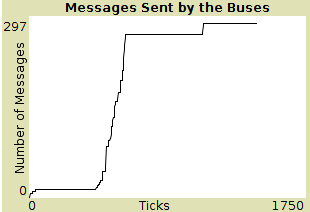
\includegraphics[width=\textwidth]{src/nr_messages.png}
  \caption{Number of exchanged messages in Day 1.}
  \label{fig:messages}
\end{minipage}
\end{figure}

\begin{figure}[htbp]
\centering
\begin{minipage}{.48\textwidth}
  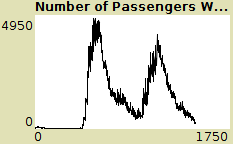
\includegraphics[width=\linewidth]{src/nr_pass_waiting.png}
  \caption{Final number of passengers waiting in Day 1.}
  \label{fig:pass_waiting}
\end{minipage}
\begin{minipage}{.48\textwidth}
  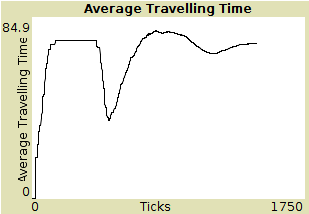
\includegraphics[width=\linewidth]{src/avg_tt.png}
  \caption{Average traveling time in Day 1.}
  \label{fig:avg_tt}
\end{minipage}
\end{figure}

Day 1 has two rush hours, in the morning and in the evening. The figures show how our solution deals with these rush hourse. First there is a peek in the number of people waiting, followed by a peek in expenses. This is due to the new buses added to manage the rush hour. During the second rush hour, the peek of people waiting is much smaller. Because the fleet is larger, the tranportation system can efficiently deal with the rush hour.

To measure performance, we check if the system is capable of handling different scenarios. The results of running the system on the training data, is compared to the results for the test data sets. Table \ref{table:table2} shows the results available for comparison.

\begin{table*}[htbp]
\centering
\begin{tabular}{ |c|c|c|  }
 \hline
  Measurement & Traning Data (Day 1) & Test Data (Day 3) & Test Data (Day 4) \\
 \hline
  Avg travelling time & 72.53 & 92.36 & 86.72 \\
  Buses' expenses & 711251 & 2393732 & 2346943.5 \\
  Messages sent & 285 & 950 & 992 \\
  Final amount waiting & 25 & 2603 & 2513 \\
  Avg travel time remaining & 78.12 & 182.97 & 206.91 \\
  Final avg travel time & 75.48 & 101.42 & 95.97 \\
 \hline
\end{tabular}
\label{table:table2}
\caption{Performance results}
\end{table*}
\begin{table*}[htbp]

The system does not perform as well on the test data, as on the training data. The average travelling time only rises a little. But the expenses and the amount of messages are tripled, because much more new buses are added. Even though the fleet was larger, the amount of people waiting in the end is larger. 

The plots using day 4 for the expenses, the messages, the number of people waiting and the travelling time are shown in Figure \ref{fig:expense4}, \ref{fig:messages4}, \ref{fig:pass_waiting4} and \ref{fig:avg_tt4} respectively. Figure \ref{fig:pass_waiting4} shows that the final amount of people waiting on day 4 is larger, even though the bus fleet is larger. It also shows that the rush hour is not properly managed. The amount of people waiting does not go down fast enough.

\begin{figure}[htbp]
\centering
\begin{minipage}{.48\textwidth}
  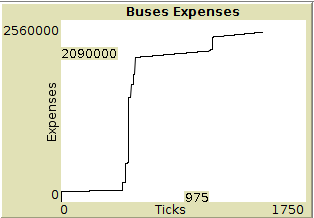
\includegraphics[width=\textwidth]{src/expenses4.png}
  \caption{Expenses of the buses in Day 4.}
  \label{fig:expense4}
\end{minipage}
\begin{minipage}{.48\textwidth}
  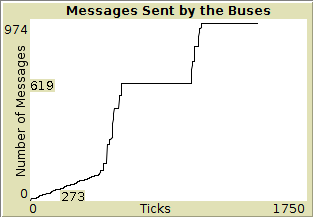
\includegraphics[width=\textwidth]{src/nr_messages4.png}
  \caption{Number of exchanged messages in Day 4.}
  \label{fig:messages4}
\end{minipage}
\end{figure}

\begin{figure}[htbp]
\centering
\begin{minipage}{.48\textwidth}
  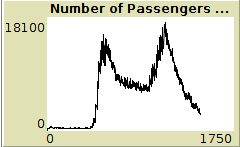
\includegraphics[width=\linewidth]{src/nr_pass_waiting4.png}
  \caption{Final number of passengers waiting in Day 4.}
  \label{fig:pass_waiting4}
\end{minipage}
\begin{minipage}{.48\textwidth}
  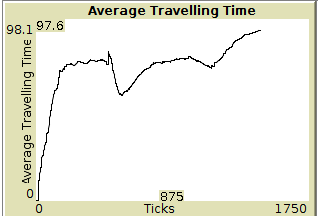
\includegraphics[width=\linewidth]{src/avg_tt4.png}
  \caption{Average travelling time in Day 4.}
  \label{fig:avg_tt4}
\end{minipage}
\end{figure}

The plots using Day 5 for the expenses, the messages, the number of people waiting and the travelling time are shown in Figure \ref{fig:expense5}, \ref{fig:messages5}, \ref{fig:pass_waiting5} and \ref{fig:avg_tt5} respectively.

\begin{figure}[htbp]
\centering
\begin{minipage}{.48\textwidth}
  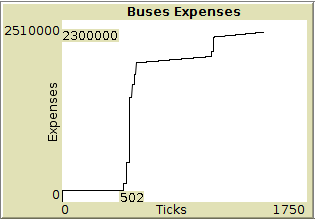
\includegraphics[width=\textwidth]{src/expenses5.png}
  \caption{Expenses of the buses in Day 5.}
  \label{fig:expense5}
\end{minipage}
\begin{minipage}{.48\textwidth}
  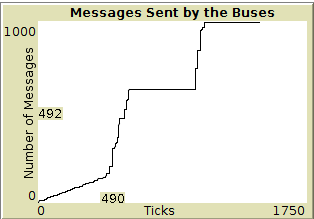
\includegraphics[width=\textwidth]{src/nr_messages5.png}
  \caption{Number of exchanged messages in Day 5.}
  \label{fig:messages5}
\end{minipage}
\end{figure}

\begin{figure}[htbp]
\centering
\begin{minipage}{.48\textwidth}
  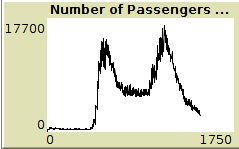
\includegraphics[width=\linewidth]{src/nr_pass_waiting5.png}
  \caption{Final number of passengers waiting in Day 5.}
  \label{fig:pass_waiting5}
\end{minipage}
\begin{minipage}{.48\textwidth}
  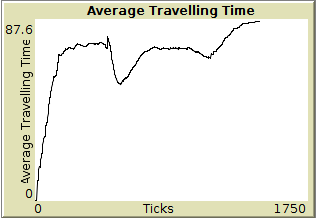
\includegraphics[width=\linewidth]{src/avg_tt5.png}
  \caption{Average travelling time in Day 5.}
  \label{fig:avg_tt5}
\end{minipage}
\end{figure}
